\documentclass[sigconf]{acmart}

\usepackage[utf8]{inputenc}
% \usepackage[hyphens]{url}
% \usepackage[pdftex,urlcolor=black,colorlinks=true,linkcolor=black,citecolor=black]{hyperref}
% \def\sectionautorefname{Section}
% \def\subsectionautorefname{Subsection}
\usepackage{graphicx}
\usepackage{caption}
\usepackage{subcaption}
\usepackage{textcomp}
\usepackage{gensymb}
\usepackage[super]{nth}
% todo macro
\usepackage{color}
\newcommand{\todo}[1]{\noindent\textcolor{red}{{\bf \{TODO}: #1{\bf \}}}}


% Copyright
%\setcopyright{none}
%\setcopyright{acmcopyright}
%\setcopyright{acmlicensed}
\setcopyright{rightsretained}
%\setcopyright{usgov}
%\setcopyright{usgovmixed}
%\setcopyright{cagov}
%\setcopyright{cagovmixed}


% DOI
\acmDOI{10.475/123_4}

% ISBN
\acmISBN{123-4567-24-567/08/06}

%Conference
\acmConference[WOODSTOCK'97]{ACM Woodstock conference}{July 1997}{El
  Paso, Texas USA}
\acmYear{1997}
\copyrightyear{2016}

\acmArticle{4}
\acmPrice{15.00}

% These commands are optional
%\acmBooktitle{Transactions of the ACM Woodstock conference}
%\ editor{Jennifer B. Sartor}
% \editor{Theo D'Hondt}
% \editor{Wolfgang De Meuter}


\begin{document}
\title[What is in a~Web View?]{What is in a~Web View?
An Analysis of Progressive Web App Features
When the Means of Web Access is not a~Web Browser}  

% \titlenote{}
% \subtitle{}
% \subtitlenote{}


\author{Thomas Steiner}
% \authornote{}
% \orcid{1234-5678-9012}
\affiliation{%
  \institution{Google Germany GmbH}
  \streetaddress{ABC-Straße 19}
  \city{20354 Hamburg}
  \country{Germany}
}
\email{tomac@google.com}

\author{Michael Yeung}
% \authornote{}
% \orcid{1234-5678-9012}
\affiliation{%
  \institution{Google Hong Kong}
  \streetaddress{1~Matheson Street}
  \city{Causeway Bay}
  \country{Hong Kong}
}
\email{micyeung@google.com}

% The default list of authors is too long for headers.
%\renewcommand{\shortauthors}{B. Trovato et al.}

\begin{abstract}
Progressive Web Apps (\textsc{pwa}) are a~new class of Web applications,
enabled for the most part by the Service Workers \textsc{api}s.
Service Workers allow apps to \emph{work offline}
by intercepting network requests to deliver programmatic or cached responses,
they can receive \emph{push notifications} and \emph{synchronize} data in the background
even when the app is not running,
and---together with Web App Manifests---allow users to \emph{install \textsc{pwa}s}
to their devices' home screens.
Service Workers being a Web standard, support has landed in several
stand-alone Web browsers---among them (but not limited to)
Chrome and its open-source foundation Chromium, Firefox, Edge, Opera,
\textsc{uc}~Browser, Samsung Internet, as well as preview versions of Safari.
In this paper, we examine the \textsc{pwa} feature support situation in \emph{Web Views},
that is,\ \emph{in-app Web experiences} that are \emph{not} stand-alone browsers.
Such in-app browsers can commonly be encountered in chat applications like WeChat or WhatsApp,
online social networks like Facebook or Twitter, but also email clients like Gmail.
We have developed an open-source application called \emph{\textsc{pwa} Feature Detector}
that allows for easily testing in-app browsers (and obviously stand-alone browsers on top)
and check for the available \textsc{pwa} features.
The results help developers make educated choices when it comes to determining
whether a~\textsc{pwa} is the right approach given their users' target means of Web access.
\end{abstract}

%
% The code below should be generated by the tool at
% http://dl.acm.org/ccs.cfm
% Please copy and paste the code instead of the example below.
%

\keywords{Progressive Web Apps, Service Workers, Web Views}

\maketitle

\section{Introduction}

In recent years, there has been a~paradigm shift
from browser to native apps and back to browser again.
The Web currently is undergoing a silent revolution with Web apps,
more descriptively \emph{Progressive Web Apps},
or for short just \textsc{pwa}s.
How did we get there?

\subsection{History of Progressive Web Apps}

Since around 2005, Web development has moved from static multi-page \emph{documents}
to single-page \emph{applications}, heavily enabled by the \texttt{XMLHttpRequest} \textsc{api},
a~process that eventually led Garrett to coin the term \emph{Ajax}
(Asynchronous JavaScript and XML~\cite{garret2005ajax}) to describe this shift.
Despite an early push for Web-based apps on devices such as the 2007 iPhone,
attempts at Web apps mostly failed by comparison to native apps
that were distributed through app stores rather than the Web.
Native apps not only had direct hardware access to, \emph{e.g.},\ camera and microphone,
to various sensors like accelerometer or geolocation, but also just in general provided
a~better user experience and booted faster compared to having to load in a~browser at runtime.
Additionally, advanced offline support and push notifications were simply unthinkable
for Web applications at the time, and Web app icons
that already could be added to devices' home screens
were mostly just bookmarks with---apart from full screen mode---no special behavior.
While straightforward offline scenarios could be realized with
\texttt{AppCache}~\cite{vankesteren2008offlinewebapps}, more complex offline scenarios were error-prone
and hard to get right~\cite{archibald2012douchebag}.

As the Web platform matured and more and more
hardware-related \textsc{api}s were implemented in browsers,
in the end it was the addition of Service Workers~\cite{russell2017serviceworkers}
to the Chromium browser in 2014~\cite{cooney2014chromium} that started to unlock a~new class of Web apps
that finally could \emph{work offline}, receive \emph{push notifications}
and \emph{synchronize} data in the background even when the app was not running,
and---together with Web App Manifests~\cite{caceres2017manifest}---allowed
users to actually \emph{install \textsc{pwa}s} to their devices' home screens
with proper operating system integration~\cite{kinlan2017a2hs}.
Other browsers like Mozilla Firefox, Microsoft Edge, Opera, \textsc{uc}~Browser, Samsung Internet,
Apple Safari Technology Preview, and several browsers more followed in implementing Service Workers.
Now, even multinational companies like Twitter
or trivago bet on \textsc{pwa}~\cite{gallagher2017twitterlite,twg2017trivago},
as well as giant national players like Tencent News or Sina Weibo in China~\cite{zhu2017pwa}.

\begin{figure}[hbt]
  \centering
  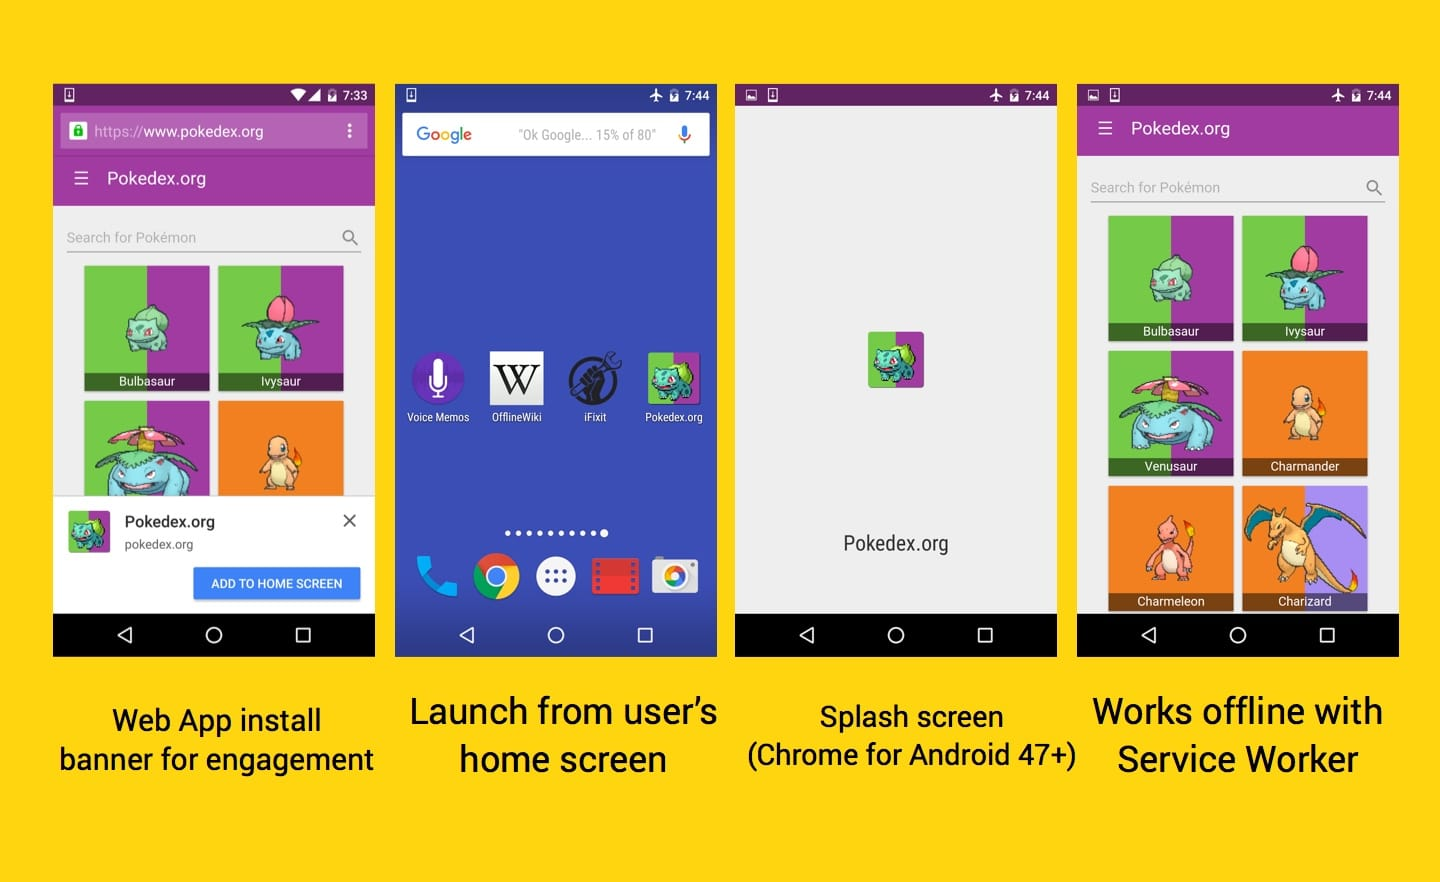
\includegraphics[width=\columnwidth]{pwa-features}
  \caption[Screenshots showing some \textsc{pwa} features]{
    Screenshots showing some \textsc{pwa} features}
    \small (\url{http://developers.google.com/web/updates/2015/12/getting-started-pwa}) 
  \label{fig:pwa-features}
\end{figure}

\subsection{Research Question and Paper Structure}

In this paper, we look at a~special means for accessing \textsc{pwa}s,
namely accessing them \emph{not} through stand-alone browsers like the ones listed above,
but through \emph{in-app browsers} that render Web content in the context of native applications.
Examples of such applications with in-app browsers are chat apps like WeChat (Wēixìn) or WhatsApp,
online social networks like Facebook or Twitter, but also email clients like Gmail.
The technology that these applications leverage internally are so-called \emph{Web Views}.
In order to understand why this presents an interesting research problem,
one needs to first understand the role that applications like WeChat play in markets like China.
Chan writes in an article~\cite{chan2015wechat} for the venture capital firm Andreessen Horowitz:
``Millions (note, not just thousands) of lightweight apps live inside WeChat,
much like webpages live on the internet.
\emph{This makes WeChat more like a~browser for mobile websites}, or, arguably,
a~mobile operating system---complete with its own proprietary app store.
The lightweight apps on WeChat are called `official accounts'.
Approved by WeChat after a~brief application process,
there are well over 10 million of these official accounts on the platform---ranging
from celebrities, banks, media outlets, and fashion brands to hospitals, drug stores,
car manufacturers, internet startups, personal blogs, and more''.
Chan goes on: ``WeChat focuses on taking care of the plumbing---overseeing
the integration of such pre-existing services into its portal---by
simply linking users from the wallet menu to webpages from within the app.
It's yet another way in which \emph{WeChat
becomes an integrated browser for the mobile (and web) world}''.
It is to be noted that this development comes to the detriment of the so-called open Web.
As Yang and Yang write in the Financial Times~\cite{yang2017tencent}:
``[WeChat's] news feed and search tools pull content only from within WeChat's walls
rather than from the open web, including updates posted by individual users called moments,
corporate accounts and an immense collection of WeChat accounts
which are used by newspapers and independent bloggers''.
While personally we are advocates of the open Web,
we therefore examine the implications of an in-app closed Web experience
and what this means for \textsc{pwa}. 

In the remainder of this paper, we first look at the technical background of Web Views
and describe the \textsc{pwa} features and their underlying \textsc{api}s in \autoref{sec:background},
introduce our application \emph{\textsc{pwa} Feature Detector} in \autoref{sec:pwa-feature-detector},
and present and discuss our results in \autoref{sec:results-and-discussion}.
We close the paper with an outlook on future work in \autoref{sec:future-work}
and draw some conclusions in \autoref{sec:conclusions}.

\section{Background on Web Views}
\label{sec:background}

There are many different ways to integrate Web content in native applications,
each having their own benefits and drawbacks.
In the following, we describe the options on the two popular
mobile operating system Android and i\textsc{os}.
At time of writing, Safari on i\textsc{os} does not support Service Workers yet.
For the sake of completeness, we nevertheless describe the Web View situation there as well.

\subsection{The Situation on Android}

\paragraph{Android Web Views with \texttt{WebView}}

In the Android operating system, a~\texttt{WebView}~\cite{android2018webview}
is a~subclass of a~\texttt{View} that displays Web pages.
This class is the basis upon which developers can create their own Web browser
or simply display some online content in their apps.
It does not include any features of a~fully developed Web browser,
such as navigation controls or an address bar.
All that \texttt{WebView} does, by default, is show a~Web page.
Therefore, it uses the system browser's rendering engine to display Web pages
and includes methods to navigate forward and backward through a history,
zoom in and out, perform text searches and more.
Looper describes~\cite{looper2015webviews}
the development of the component as follows:
``Whereas earlier versions of the Android \textsc{os}
relied on the WebKit rendering engine to power its \texttt{WebView},
as of Android~4.4, various versions of Chromium are implemented.
Typically, with each consecutive update of Android's \texttt{os},
a~new version of Chromium would also be included, thereby giving access
to the new rendering engine's capability.
This causes issues in backward compatibility for developers
who must support earlier versions of Android.
To combat this particular problem, as of Android~5.0,
the concept of the auto-updating \texttt{WebView} has been introduced.
Instead of the \texttt{WebView} version and capabilities
depending on Android \textsc{os}' update cycle,
the Android~5.0 \texttt{WebView} is a~system-level \texttt{.apk} file
available in Google Play that can update itself in the background''.

\paragraph{Chrome Custom Tab with \texttt{CustomTabsIntent}}

While \texttt{WebView}s are completely isolated from the user's regular browsing activities,
Chrome Custom Tabs~\cite{kinlan2016customtabs}, available since Chrome~45 (September 2015)
and instantiatable as \texttt{CustomTabsIntent}, provide a~way for an application
to customize and interact with a~Chrome Activity on Android.
This makes the Web content feel like being a part of the application,
while retaining the full functionality and performance of a~complete Web browser
through a~shared cookie jar and permissions model, so users do not have to log in
to sites they are already connected to, or re-grant permissions they have already granted.

\paragraph{Trusted Web Activity with \texttt{TwaSessionHelper}}

Chrome Custom Tabs solved many issues of Android Web Views,
however, had the drawback of not being available in a~fullscreen variant like Web Views.
As of October 2017, Trusted Web Activities~\cite{googledevelopers2017twa} are a~new way to
integrate Web app content such as \textsc{pwa}s with Android apps.
They can be instantiated with a~\texttt{TwaSessionHelper}
and use a~protocol based on Chrome Custom Tabs.
Content in a~Trusted Web Activity is trusted---the app and the site it opens
are expected to come from the same developer, this is verified using Digital Asset
Links.\footnote{Digital Asset Links:
\url{https://developers.google.com/digital-asset-links/}}
The host app does not have direct access to Web content in a~Trusted Web Activity
or any other kind of Web state.
Transitions between Web and native content are between activities.
Each activity (\emph{i.e.},\ screen) of an app is either completely provided by the Web,
or by an Android activity.
While not enforced at time of writing, Trusted Web Activities
will ultimately need to meet content requirements
similar to the ``improved add to home screen`` flow~\cite{kinlan2017a2hs},
which is designed to be a~baseline of interactivity and performance.

\subsection{The Situation on i\textsc{os}}

\paragraph{i\textsc{os} Web Views with \texttt{UIWebView}}

Similar to Android, on i\textsc{os} as well Web content could be embedded with
a~simple system-level Web View called \texttt{UIWebView}.\footnote{\texttt{UIWebView}:
\url{https://developer.apple.com/library/ios/documentation/UIKit/Reference/UIWebView_Class/}}
With the release of i\textsc{os}~4.3 in early 2011, Apple introduced Nitro,
a~faster, just-in-time (\textsc{jit}) JavaScript engine for Safari
that considerably sped up the browser's performance in loading complex Web pages.
Nitro was exclusive to Safari: third-party developers could not benefit
from the faster performance in their Web views based on \texttt{UIWebView},
which was widely considered a~calculated move to encourage usage of Safari
over Web Views and Web apps saved to the iPhone's home screen~\cite{viticci2015safari}.

\paragraph{i\textsc{os} Web Views with \texttt{WKWebView}}

In June 2014, Apple announced \texttt{WKWebView},\footnote{\texttt{WKWebView}:
\url{https://developer.apple.com/library/ios/documentation/WebKit/Reference/WKWebView_Ref/}}
a~new API that would allow developers
to display Web content in custom Web Views with the same performance benefits of Safari.
Designed with security in mind, \texttt{WKWebView} featured the same Nitro engine of Safari,
while still allowing developers to customize the experience
with their own user interface and features.
Due to Apple's App Store restrictions, third-party browsers on i\textsc{os}
internally need to depend on \texttt{WKWebView}, documented,
\emph{e.g.},\ for Edge for i\textsc{os}~\cite{lyndersay2017edge}
or Chrome for i\textsc{os}~\cite{chromiumblog2016chrome}.

\paragraph{i\textsc{os} Web Views with \texttt{SFSafariViewController}}

In September 2015 with the release of i\textsc{os}~9, Apple introduced a~new Web View called
\texttt{SFSafariViewController}\footnote{\texttt{SFSafariViewController}:
\url{https://developer.apple.com/documentation/safariservices/sfsafariviewcontroller}},
which enables apps to delegate the responsibility of showing Web content to Safari itself,
avoiding the need to write custom code for built-in browsers.
Up until i\textsc{os}~10, Safari View Controller shared cookies and website data with Safari,
which means that if a~user was already logged into a~specific website in Safari
and a~link to that website was opened in Safari View Controller,
the user was already logged in.
As of i\textsc{os}~11, cookie and website data is no longer shared,
but developers can leverage
an \texttt{SFAuthenticationSession}\footnote{\texttt{SFAuthenticationSession}:
\url{https://developer.apple.com/documentation/safariservices/sfauthenticationsession}}
that shares data upon user consent. 

\subsection{Parallelisms on the Two Operating Systems}

The development on the two operating systems has certain parallels
that can be summarized as follows.
From the initially slow and gradually improved simple Web Views \texttt{WebView}
(with the transparent internal switch from WebKit to Chromium)
on Android and \texttt{UIWebView} and \texttt{WKWebView} on i\textsc{os},
there was an evolution to more powerful and better integrated browser tab experiences,
namely \texttt{CustomTabsIntent} on Android and
\texttt{SFSafariViewController} on i\textsc{os},
which both (only upon user consent since i\textsc{os}~11)
share cookies, permissions, \emph{etc.}
with the particular system's main browser.
Android's \texttt{TwaSessionHelper} so far has no i\textsc{os} equivalent yet.

\section{\textsc{pwa} Feature Detector}
\label{sec:pwa-feature-detector}

What exactly makes a~Web app a~\emph{Progressive} Web App is not clearly defined.
One of the most open definitions comes from Samsung~\cite{samsung2017pwa},
maker of the Samsung Internet browser (emphasis ours):
``Progressive Web Apps (\textsc{pwa}s) are regular mobile and desktop web applications
that are accessible in any web browser.
In browsers that support new open web standards [\ldots]
they \emph{can} provide additional capabilities
including offline support and push notifications.''
However, just like with Ajax~\cite{garret2005ajax}, the term \textsc{pwa}
became a~catch-all umbrella brand for Web apps
that in some way or the other use Service Worker \textsc{api}s,
feel (native) ``app-like,'' use latest browser features if they are available
(Progressive Enhancement~\cite{champeon2003progressiveenhancement}),
or that can be installed (added) to the home screen.
Russell~\cite{russell2016pwa} lists a~number of requirements 
for what he calls ``baseline appyness'':
``A~Progressive Web App is functionally defined by the technical properties
that allow the browser to detect that the site meets certain criteria
and is worthy of being added to the homescreen.
These criteria are motivated by user-experience concerns.
Apps on the homescreen:

\subsection{Progressive Web App Features}

\begin{enumerate}
  \item Should load instantly, regardless of network state.
    This isn't to say that they need to function fully offline,
    but they must put their own UI on screen without requiring a network round trip.
  \item Should be tied in the user's mind to where they came from.
    The brand or site behind the app shouldn't be a mystery.
  \item Can run without extra browser chrome (\emph{e.g.},\ the \textsc{url} bar).
    This is a~potentially dangerous permission.
    To prevent hijacking by captive portals (and worse),
    apps must be loaded over \textsc{tls} connections.''
\end{enumerate}

Translated to technical terms, Russell's definition implies that \textsc{pwa}s must:

\begin{enumerate}
  \item ``Originate from a Secure Origin.
    Served over TLS and green padlock displays (no active mixed content).
  \item Load while offline (even if only a custom offline page).
    By implication, this means that Progressive Web Apps require Service Workers.
  \item Reference a~Web App Manifest [\ldots]''
\end{enumerate}


%
%     'Offline Capabilities': 'caches' in win,
%      'Push Notifications': 'pushManager' in registration,
%      'Add to Home Screen': 'BeforeInstallPromptEvent' in win,
%      'Background Sync': 'sync' in registration,
%      'Navigation Preload': 'navigationPreload' in registration,
%      'Budget API': 'budget' in nav && 'reserve' in nav.budget,
%      'Storage Estimation': 'storage' in nav && 'estimate' in nav.storage,
%      'Persistent Storage': 'storage' in nav && 'persist' in nav.storage,
%      'Web Share': 'share' in nav,
%      'Media Session': 'mediaSession' in nav,
%      'Media Capabilities': 'mediaCapabilities' in nav,
%      'Device Memory': 'deviceMemory' in nav,
%      'Getting Installed Related Apps': 'getInstalledRelatedApps' in nav,
%      'Payment Request': 'PaymentRequest' in win,
%      'Credential Management': 'credentials' in nav,

\subsection{Feature-Detecting Various Features}

\subsection{Implementation Details}

\section{Results and Discussion}
\label{sec:results-and-discussion}

\section{Future Work}
\label{sec:future-work}

\section{Conclusions}
\label{sec:conclusions}


\bibliographystyle{ACM-Reference-Format}
\bibliography{bibliography}

\end{document}
